\section{Experiments}
\label{sec:experiments}

\subsection{Experimental Setup}

\subsubsection{Research Objectives}
The objective of this study is to evaluate the effectiveness of the proposed \textbf{MR-CDM} model for time series forecasting tasks. Specifically, the experiments are designed to:
(1) verify the effectiveness of multi-scale trend decomposition in improving forecasting accuracy;
(2) evaluate the performance of conditional diffusion models in time series forecasting;
(3) analyze the effectiveness of transforming time series into image representations; and
(4) compare traditional time series forecasting methods with diffusion-based approaches.

\subsubsection{Experimental Environment}
All experiments were conducted on a high-performance workstation configured with an Intel Xeon Silver 4110 CPU, 256 GB of DDR4 RAM, and two NVIDIA TITAN RTX GPUs, each equipped with 24 GB of dedicated memory. The software stack was built on Ubuntu 20.04 LTS and included Python 3.11, PyTorch 2.0.1, and CUDA 11.8 to enable efficient GPU-accelerated training and inference. This setup ensured consistent and reproducible experimental conditions across all evaluations.

\subsubsection{Evaluation Metrics}
We adopt three primary evaluation metrics: Mean Squared Error (MSE), Mean Absolute Error (MAE), and Root Mean Squared Error (RMSE), which measure the squared error, absolute error, and scale-consistent error between predictions and ground truth, respectively. 

\subsection{Datasets and Preprocessing}

\subsubsection{Dataset Description}
Experiments are conducted on the ETTh1 (Electricity Transformer Temperature - Hourly) dataset. The dataset spans from July 2016 to July 2018 with an hourly sampling rate, containing 17,420 time points and seven features. Following common practice, we focus on the univariate forecasting task of the LUFL variable. 
% The demonstration of our model's adaptability in other fields is provided in Appendix~\ref{sec:Generalization} in our paper.
The demonstration of our model's adaptability in other fields is provided in Appendix~B in our technique paper~\cite{Xu2026MRImaginTime}.

\subsubsection{Data Preprocessing}
Data preprocessing consists of three main steps. First, missing values are filled using linear interpolation, and outliers are detected and handled based on the $3\sigma$ rule to ensure temporal continuity. Second, Z-score normalization is applied using statistics computed from the training set:
\[x_{\text{norm}} = \frac{x - \mu}{\sigma}.\]
Finally, the dataset is split chronologically into training (70\%), validation (10\%), and testing (20\%) sets, corresponding to 12,194, 1,742, and 3,484 time points, respectively.

\subsubsection{Dataset Sythesis}
To demonstrate the generalization capability in similar dataset of our model, we generated a synthetic dataset using a multi-component time series synthesis approach. The synthetic data preserves the statistical properties (mean, standard deviation, and value ranges) of the original ETTh1 dataset while incorporating realistic temporal patterns including daily cycles (24-hour periodicity), weekly cycles (7-day periodicity), long-term trends, and Gaussian noise. Inter-variable correlations were maintained through correlated signal generation, and daytime load enhancement was applied to simulate realistic power consumption patterns. 


\subsection{Baseline Models}

% \subsubsection{Traditional Time Series Model}
%  ARIMA serves as a representative baseline for univariate forecasting tasks, offering strong performance on stationary or weakly non-stationary series without requiring deep learning infrastructure.This automated selection process allows for a fair and data-driven comparison against more complex modern approaches.The ARIMA baseline model adopts the standard ARIMA(2,1,2) configuration. During the prediction process, the average trend is calculated based on the last 10 values of the historical sequence, and a linear extrapolation is performed to generate 96-step predictions. Additionally, Gaussian noise based on the historical variance is added to simulate the uncertainty of the prediction. It is a standard configuration in time series prediction, balancing model complexity and generalization ability, and is suitable for most non-stationary time series.
% \subsubsection{Deep Learning Baseline}
% We adopt a two-layer LSTM (Long Short-Term Memory) network as a deep learning baseline for sequence modeling. This architecture provides a strong and widely used benchmark for neural time series forecasting, capturing temporal dependencies through gated recurrent dynamics while remaining computationally efficient. As such, it serves as a meaningful reference point against which more advanced or specialized models can be evaluated.We adopt a two-layer stacked LSTM architecture, with a hidden layer size of 128 (consistent with the base channel number of the U-Net in MR-CDM), and a dropout rate of 0.2 to prevent overfitting. The model takes the hidden state of the last time step as the input and outputs the predicted values for 96 steps through a fully connected layer. Training uses the AdamW optimizer with a learning rate of 0.0001, weight decay of 0.00001, batch size of 16, and trains for 200 epochs. It employs cosine annealing learning rate scheduling and gradient clipping (maximum norm 1.0).
% \subsubsection{Advanced Diffusion Model}
% CSDI is a conditional score-based diffusion model initially developed for imputation but widely applicable to forecasting. It adopts a score matching framework rather than standard noise prediction, allowing for more accurate learning of data distribution gradients and higher-fidelity sample generation. Then CSDI employs a masking mechanism to explicitly separate observed history from future targets, enabling powerful conditional generation that outperforms unconditional variants in capturing temporal dependencies. Using 6 layers of residual blocks, each layer consists of causal convolution and multi-head self-attention, with a hidden dimension of 64 channels and 4 multi-heads.And its architecture combines causal convolutions and multi-head self-attention to jointly model local temporal dynamics and global feature interactions. 
\subsubsection{Traditional Time Series Model}
We adopt ARIMA(2,1,2) as a standard univariate baseline, suitable for non-stationary series. It performs 96-step prediction via linear extrapolation of the recent trend, augmented with Gaussian noise to model uncertainty.

\subsubsection{Deep Learning Baseline}
A two-layer stacked LSTM with 128 hidden units and 0.2 dropout serves as our deep learning baseline. It generates 96-step forecasts from the final hidden state. We train for 200 epochs using AdamW (lr=0.0001, weight decay=0.00001), with cosine annealing and gradient clipping (max norm 1.0).

\subsubsection{Advanced Diffusion Model}
We utilize CSDI, a conditional score-based diffusion model for forecasting. It employs a masking mechanism for conditional generation and uses 6 residual blocks (causal convolutions + 4-head self-attention, hidden dim=64) to model both local and global temporal dependencies.

\subsection{Implements Details of Feature Processing}
\textbf{Multi-scale Trend Decomposition.} 
In the decomposition stage, we employ three moving average filters with window sizes of $[5, 25, 51]$, corresponding to temporal scales of approximately 5 hours, 1 day, and 2 days, respectively. This configuration enables the capture of multi-level features ranging from short-term fluctuations to long-term trends. Specifically, the filter with window size 5 (MA-5) extracts high-frequency short-term fluctuations, MA-25 identifies daily periodic patterns, and MA-51 captures long-term trends. This hierarchical design ensures that features at distinct temporal scales are disentangled and can be subjected to differentiated processing strategies.

\textbf{Adaptive Image Transformation.} 
For the components $\text{Trend}_1$, $\text{Trend}_2$, and the $\text{Residual}$, we utilize the delay embedding method to transform 1D time series into $32 \times 32$ 2D images, setting the delay parameter $\tau=3$ and the embedding dimension $d=32$. Here, $\tau=3$ effectively captures temporal dependencies over a 3-hour span, while $d=32$ aligns with the base resolution of the U-Net architecture, thereby avoiding unnecessary upsampling or downsampling operations. Conversely, for $\text{Trend}_3$, we apply the Short-Time Fourier Transform (STFT) to convert the signal into the time-frequency domain, configured with $\text{n\_fft}=64$ and $\text{hop\_length}=16$. The choice of $\text{n\_fft}=64$ yields 32 frequency components sufficient for identifying periodic characteristics, while $\text{hop\_length}=16$ ensures a 75\% window overlap, guaranteeing temporal continuity and information integrity.

\textbf{Image Fusion.} 
In the fusion stage, we adopt a channel concatenation strategy to merge the images of the four components into a single fused tensor with 35 channels (structured as $7+7+14+7$). This design preserves the complete information of all components, facilitating subsequent hierarchical reconstruction.
\subsection{Main Results}

\subsubsection{Overall Performance Comparison}

Table~\ref{tab:main_results} reports the forecasting performance on the ETTh1 LUFL task on these models above.

\begin{table}[h]
\centering
\caption{Performance comparison on ETTh1}
\label{tab:main_results}
\begin{tabular}{lcccc}
\hline
Model & MSE & MAE & RMSE\\
\hline
ARIMA & {42.2121} & {6.2893} & {6.496}\\
LSTM & {13.4981} & {3.6270} & {3.6739}\\
CSDI & {1.5538} & {0.8992} & {1.2465}\\
MR-CDM & {1.4842} & {0.9650} & {1.2183}\\
\hline
\end{tabular}
\end{table}

\begin{figure}
	\raggedleft           
	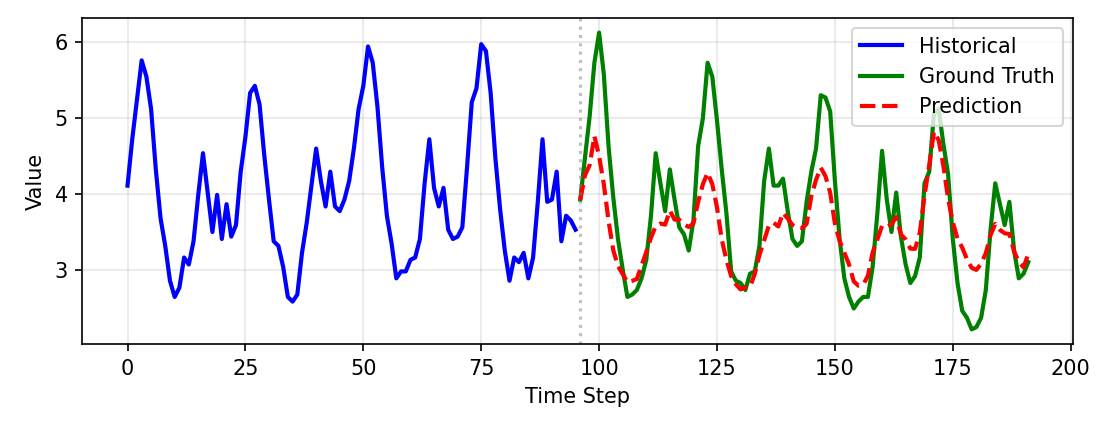
\includegraphics[width=\linewidth]{figures/prediction.eps}
	\caption{The Prediction Result Based on Our MR-CDM Model
	}
	\label{fig:result}
\end{figure}

% As shown in Table~\ref{tab:main_results},we conducted comparative experiments against two representative baseline models and advanced diffusion model on the ETTh1 feature prediction task. Our proposed MR-CDM achieves superior performance with a remarkable 96.5 percent MSE reduction compared to ARIMA and 89.0 percent improvement over LSTM.  Although the prediction result has been improved by CSDI compared with LSTM and ARIMA, our model performances better than CSDI. These substantial performance gaps demonstrate that our approach captures complex temporal patterns that traditional statistical methods and standard deep learning approaches fail to, validating the effectiveness of explicitly modeling hierarchical trend structures for time series forecasting.
As shown in Table~\ref{tab:main_results}, we compare MR-CDM with two representative baselines and an advanced diffusion model on the ETTh1 feature prediction task. MR-CDM achieves superior performance, with a 96.5 percent MSE reduction compared to ARIMA and an 89.0 percent improvement over LSTM. Although CSDI outperforms ARIMA and LSTM, our model further surpasses CSDI. These results indicate that MR-CDM more effectively captures complex temporal patterns, highlighting the importance of explicitly modeling hierarchical trends.

% As illustrated in \autoref{fig:result}, the prediction performance of the MR-CDM model on long-term LUFL forecasting is evaluated using the ETTh1 dataset. The horizontal axis denotes the time steps, covering a total duration of 192 hours (i.e., 8 consecutive days) with hourly sampling resolution. Specifically, the first 96 time steps (indexed from 0 to 95) constitute the historical input sequence—serving as the contextual basis for the model’s inference—while the subsequent 96 time steps (indexed from 96 to 191) represent the multi-step-ahead prediction horizon. 
As illustrated in \autoref{fig:result}, we evaluate the prediction performance of MR-CDM on long-term LUFL forecasting using the ETTh1 dataset. The input sequence consists of the first 96 time steps (0–95), while the subsequent 96 steps (96–191) form the prediction horizon, covering a total duration of 192 hours (8 days) with hourly resolution.

% 没有精简The vertical axis displays the LUFL values after inverse normalization, which span approximately from 2.5 to 6.0, reflecting the actual operational range of the target variable. A prominent vertical dashed line at time step 96 clearly demarcates the boundary between the observed historical data and the model-generated forecasts, thereby offering a visual distinction between known inputs and predicted outputs. This visualization not only highlights the temporal continuity and smoothness of MR-CDM’s predictions but also underscores its capability to capture long-range dependencies and maintain forecast fidelity over an extended horizon.

% Experimental results on ETTh1 confirm that MR-CDM outperforms CSDI as shown in \autoref{fig:csdi_result}. This superiority stems from fundamental architectural differences. MR-CDM explicitly decomposes time series into short-term, mid-term, and long-term components, applying specialized strategies like delay embedding and STFT for each scale, whereas CSDI relies on a unified causal convolution that blurs multi-scale features,which is interpreted in the result table. By mapping these components to the image domain via adaptive transformation, MR-CDM leverages diffusion strengths in structured data generation, unlike CSDI’s direct operation in raw time-series space.Furthermore, its multi-path hierarchical reconstructor—integrating hierarchical recovery, cross-scale attention, and adaptive weighting—precisely captures inter-scale interactions, surpassing CSDI’s single-path decoder. This targeted multi-scale design enables more efficient feature learning and higher fidelity in modeling complex temporal dynamics.
Experimental results on ETTh1 further confirm that MR-CDM outperforms CSDI, as shown in \autoref{fig:csdi_result}. This advantage arises from key architectural differences. MR-CDM explicitly decomposes time series into multi-scale components and applies tailored strategies such as delay embedding and STFT, whereas CSDI relies on a unified convolution that limits multi-scale representation. By transforming time series into the image domain, MR-CDM better leverages diffusion-based generation. In addition, its multi-path hierarchical reconstructor captures inter-scale dependencies more effectively than CSDI’s single-path decoder, leading to improved feature learning and prediction accuracy.

\begin{figure}
	\raggedleft           
	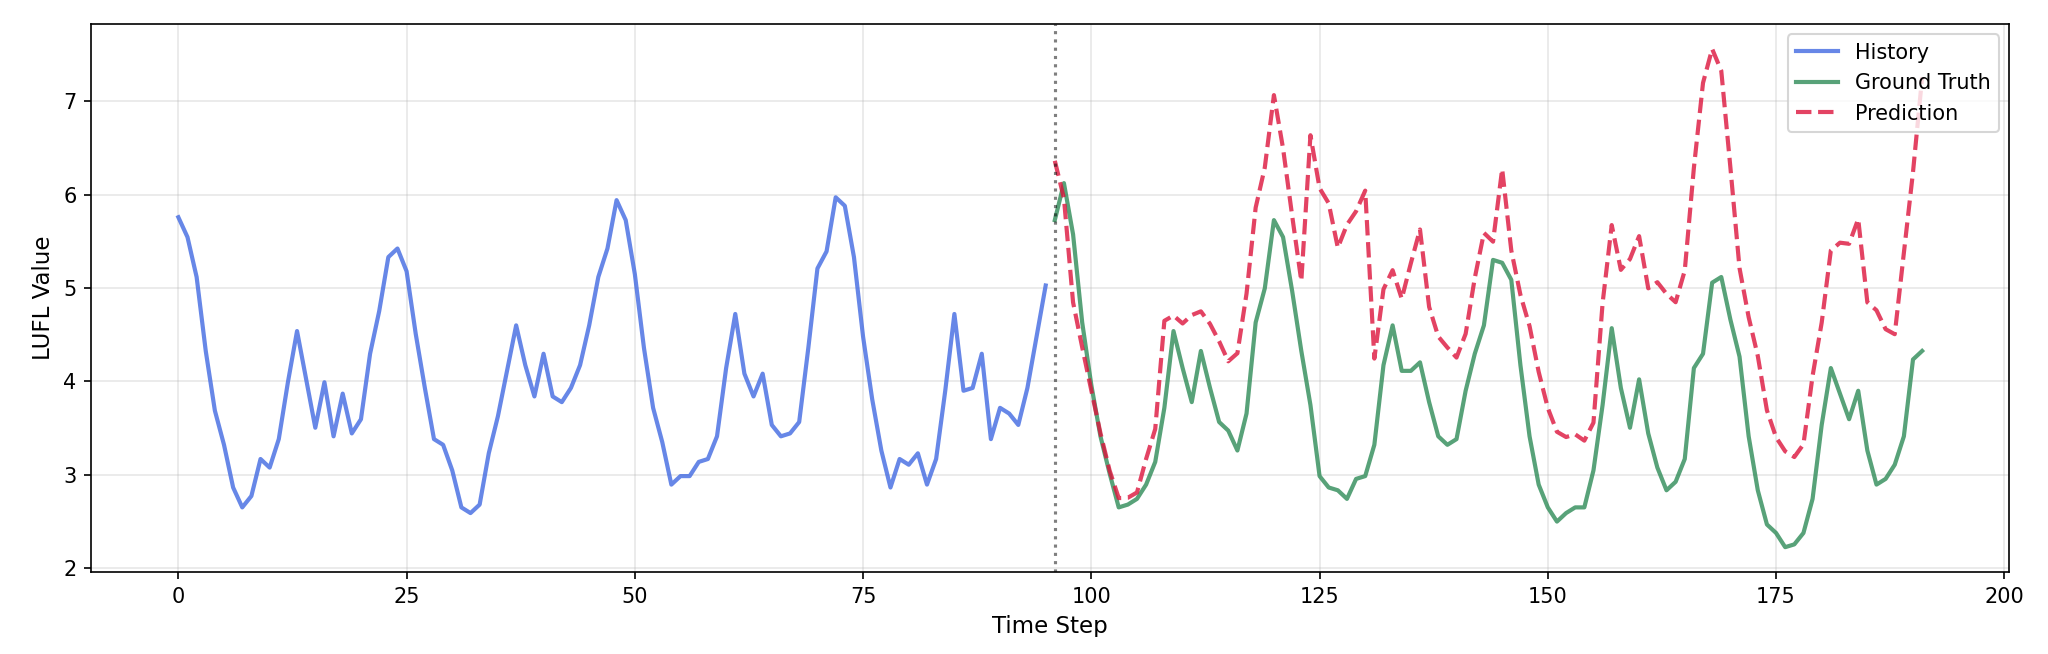
\includegraphics[width=\linewidth]{figures/csdi_prediction.eps}
	\caption{The Prediction Result Based on CSDI Model
	}
	\label{fig:csdi_result}
\end{figure}

% The blue solid line represents the historical LUFL sequence, exhibiting characteristic periodic patterns with regular oscillations and varying amplitudes, reflecting the typical daily and weekly load patterns in electrical systems. The green solid line shows the ground truth values for the prediction period, maintaining similar periodic behavior with peak values around 6.0 and trough values near 2.5. The red dashed line depicts predictions, which demonstrate remarkable alignment with the ground truth trajectory. Notably, the model successfully captures both the overall trend and the fine-grained periodic fluctuations throughout the 96-hour prediction horizon. The predictions closely follow the ground truth peaks and valleys, with particularly accurate performance in capturing the amplitude variations and phase alignment of the cyclical patterns. 

\begin{table}[h]
\centering
\caption{Performance comparison on Sythetic Dataset}
\label{tab:main_results_systhetic}
\begin{tabular}{lccc}
\hline
Model & MSE & MAE & RMSE\\
\hline
ARIMA & {39.8131} & {8.3046} & {6.3097}\\
LSTM & {12.7953} & {8.2361} & {3.5770}\\
CSDI & {1.6749} & {0.8741} & {1.2941}\\
MR-CDM & {1.2544} & {0.9080} & {1.1200}\\
\hline
\end{tabular}
\end{table}

% To further validate the robustness and generalizability of our approach, we conducted identical experiments on a synthetically generated dataset that closely mimics the statistical properties, multi-scale periodicity, and inter-variable correlations of the original ETTh1 data, as shown in \autoref{tab:main_results_systhetic}. The consistent and substantial gains on both real and synthetic data confirm that our framework is not merely overfitting to idiosyncrasies of the original dataset but genuinely captures the underlying temporal dynamics through its explicit modeling of hierarchical trend structures. This result strongly supports the effectiveness and transferability of integrating multi-scale decomposition with conditional diffusion mechanisms for time series forecasting across diverse data distributions.
To further validate robustness and generalization, we conduct the same experiments on a synthetic dataset with similar statistical properties, multi-scale periodicity, and correlations as ETTh1, as shown in \autoref{tab:main_results_systhetic}. The consistent improvements on both real and synthetic data demonstrate that MR-CDM does not overfit specific datasets but effectively captures underlying temporal dynamics. This validates the generalizability of combining multi-scale decomposition with conditional diffusion for time series forecasting.

 % A rigorous multiple-run validation protocol was employed to mitigate the impact of random variation and ensure fair comparison.  Appendix~\ref{sec:multiple} in our paper presents the comprehensive statistical summaries, confirming the reliability of our experimental setup and the consistent performance patterns across runs.
 Appendix~C in our technique paper~\cite{Xu2026MRImaginTime} presents the comprehensive statistical summaries, confirming the reliability of our experimental setup and the consistent performance patterns across runs.
% \subsubsection{Multiple-Run Validation}
% To ensure the robustness and reproducibility of our results, each experiment is repeated three times using distinct random seeds (specifically, 42, 43, and 44). This practice helps account for the inherent stochasticity in model initialization and training dynamics. The corresponding statistical summaries—including mean and standard deviation of key performance metrics across the three runs—are reported in \autoref{tab:multiple-run}(ETTh1) and \autoref{tab:multiple-run-sythetic}(Synthetic ETTH1). These aggregated results provide a more reliable basis for comparison and mitigate the influence of random variation on our conclusions.

% \begin{table}[h]
% \centering
% \caption{Multiple-Run Performance on ETTh1}
% \label{tab:multiple-run}
% \begin{tabular}{lccc}
% \hline
% Model & MSE & MAE & RMSE \\
% \hline
% ARIMA & {30.0946} & {8.2296} & {5.4858}\\
% LSTM &  {13.2883} & {6.2361} & {3.6453}\\
% CSDI & {2.7493} & {1.2478} & {1.6581}\\
% \hline
% \end{tabular}
% \end{table}
% To ensure the reliability and reproducibility of our experimental results, we conducted multiple-run validation for all baseline models. Specifically, we trained and evaluated ARIMA,LSTM and CSDI models three times with different random seeds, and reported the averaged performance metrics across all runs. This rigorous validation protocol helps mitigate the impact of random initialization and stochastic training processes, providing more robust and statistically reliable comparisons. The results presented in \autoref{tab:multiple-run} show the mean performance across three independent runs. These averaged results demonstrate consistent performance patterns across multiple runs, confirming the stability of baseline model performance and ensuring fair comparison with our proposed method. The relatively small variance across runs (not shown for brevity) further validates the reliability of our experimental setup and the robustness of the reported performance improvements.

% \begin{table}[h]
% \centering
% \caption{Multiple-Run Performance on Synsetic ETTh1}
% \label{tab:multiple-run-sythetic}
% \begin{tabular}{lccc}
% \hline
% Model & MSE & MAE & RMSE \\
% \hline
% ARIMA & {47.2826} & {7.4434} & {6.8762}\\
% LSTM &  {13.6146} & {3.6670} & {3.6897}\\
% CSDI & {2.6159} & {1.9632} & {1.6173}\\
% \hline
% \end{tabular}
% \end{table}
% Similarly, we also repeated the aforementioned baseline experiments on the synthetic dataset three times, using different random seeds to account for stochastic variations in model initialization and training. The results across all runs demonstrate consistent performance for ARIMA, LSTM and CSDI baseline models, confirming their stability on this controlled dataset. As shown in the corresponding evaluation metrics reported in the relevant \autoref{tab:multiple-run-sythetic}, the low variance across repetitions further validates the reliability of these baselines under synthetic conditions. These findings not only reinforce the robustness of our experimental setup but also provide a solid foundation for comparing more advanced methods, thereby supporting our overall analysis and conclusions.

% Experiments demonstrate that MR-CDM significantly outperforms baselines. Experiments studies attribute this gain to three core mechanisms: multi-scale trend decomposition disentangles short-, mid-, and long-term components for independent feature learning, surpassing ARIMA’s linearity,LSTM’s monolithic encoding and CSDI's instability; conditional diffusion injects historical context to ensure temporal continuity, yielding higher accuracy than unconditional generation; and a multi-path hierarchical reconstructor leverages parallel pathways (hierarchical recovery, cross-scale attention, adaptive weighting) to precisely restore details, avoiding LSTM’s gradient vanishing and information loss. Crucially, the complete framework exhibits strong synergistic effects, where the integrated performance exceeds the sum of individual contributions, validating the necessity of the proposed architecture.


\begin{figure}[htbp]
	\raggedleft           
	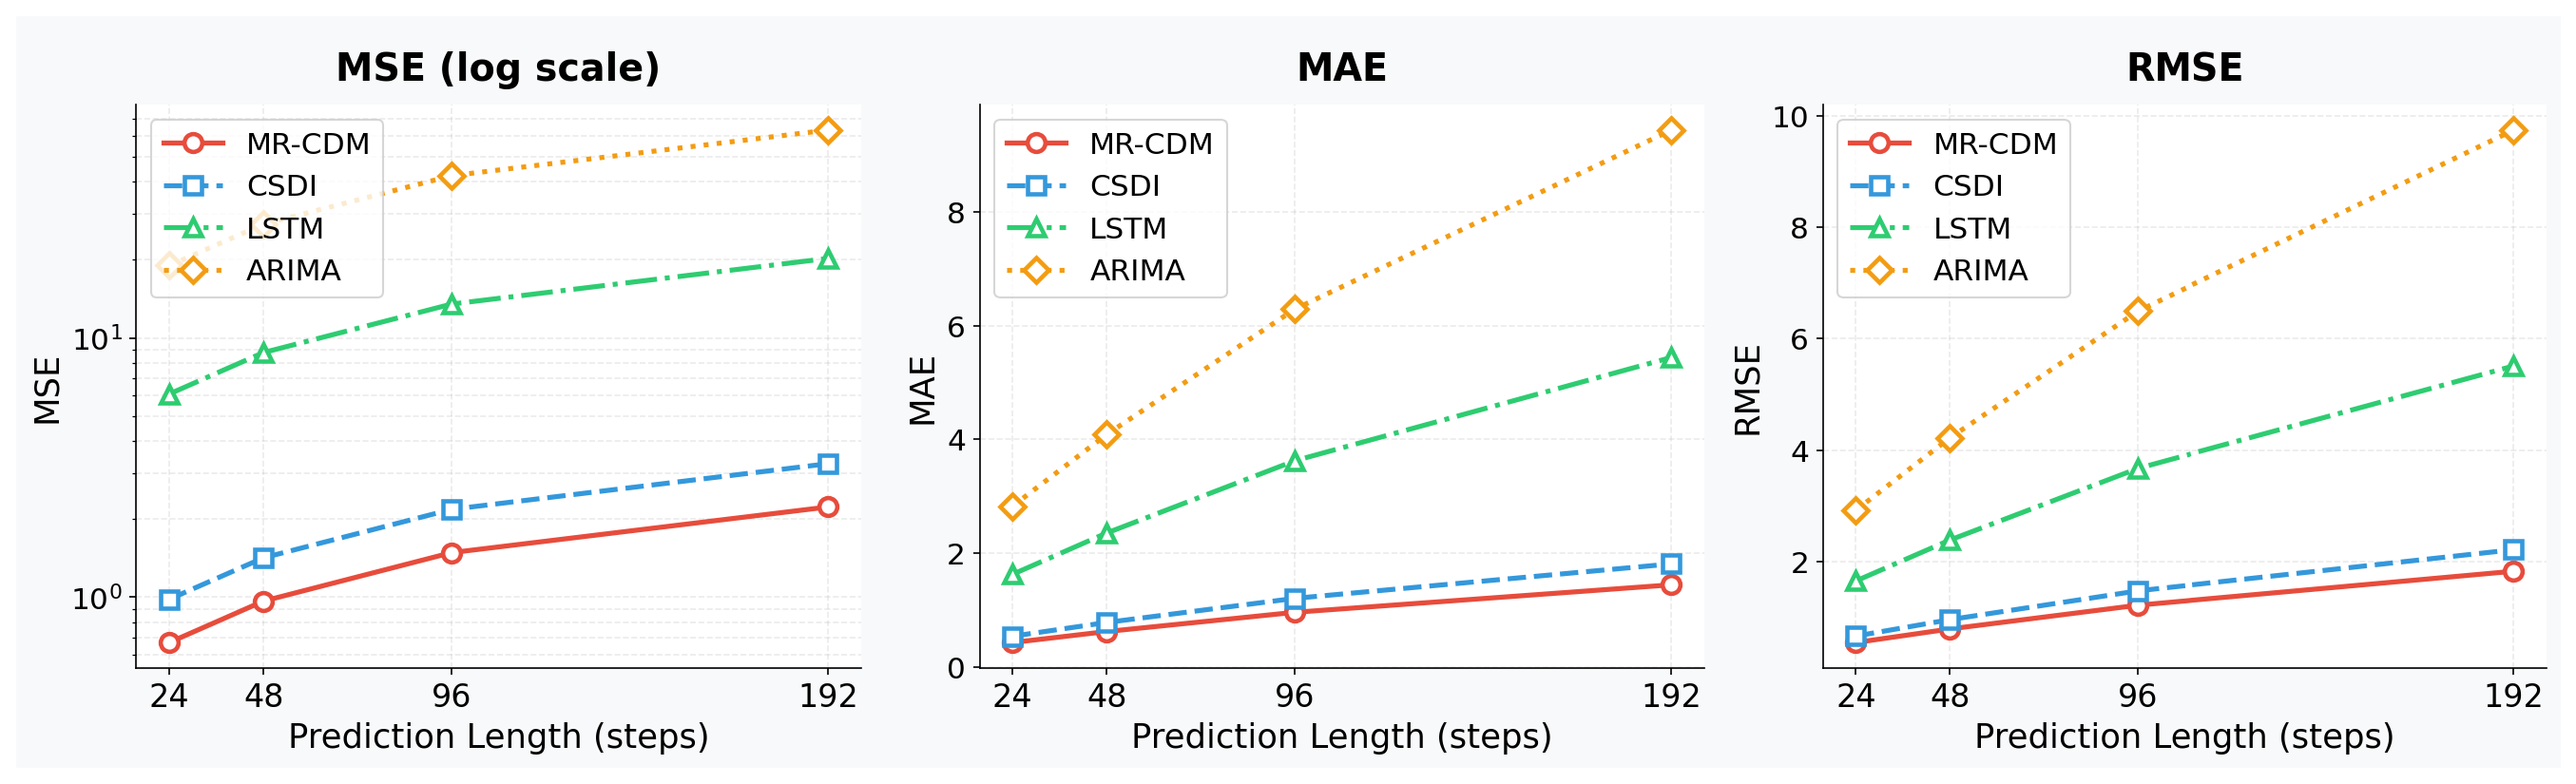
\includegraphics[width=\linewidth]{figures/exp1_preview_logscale.eps}
	\caption{Multi-Step Prediction Performance Comparison}
	\label{fig:multisteps}
\end{figure}

To evaluate the multi-step forecasting performance of MR-CDM on time series data, we conduct a comprehensive comparison experiment on the ETTh1 dataset. The historical input window is fixed at 96 time steps, while the prediction horizon is varied across four settings: 24, 48, 96, and 192 steps, enabling a systematic assessment of model accuracy and error degradation under increasing forecasting difficulty, as shown in \autoref{fig:multisteps}. Three baseline models are selected for comparison: ARIMA, LSTM, and CSDI. As illustrated in the figure, MR-CDM consistently achieves the lowest error across all prediction horizons, and its error growth rate remains significantly lower than that of the baselines as the prediction length increases. These results demonstrate that MR-CDM effectively suppresses error accumulation in long-range forecasting scenarios, confirming the superiority of the proposed approach for multi-step time series prediction tasks.



% \subsection{Generalization to Other Domains}
% To further validate the generalization capability and robustness of our model, we extended our evaluation to datasets from distinct domains: weather forecasting and traffic flow prediction. These datasets embody complex non-linear spatiotemporal dynamics characteristic of meteorological variations and urban traffic patterns, respectively, thereby serving as rigorous benchmarks for assessing cross-domain adaptability.In our experiments, the OT metric serves as the ground truth for forecasting tasks on both datasets. Experimental results demonstrate that our model not only retains its performance advantages but also achieves superior prediction accuracy and stability in these diverse scenarios, underscoring its significant potential for broad real-world applications.\autoref{tab:weather} and \autoref{tab:traffic} show the prediction ability among these models.


% Weather dataset comprises 21 multivariate time series collected from a meteorological station in Jena, Germany, with a sampling rate of 10 minutes. Characterized by complex seasonal patterns (daily and yearly cycles) and high-frequency noise, this dataset tests the model's robustness in handling non-stationary environmental data and capturing inter-variable dependencies.


% \begin{table}[h]
% \centering
% \caption{Model Performance on Weather Domain}
% \label{tab:weather}
% \begin{tabular}{lccc}
% \hline
% Model & MSE & MAE & RMSE \\ \hline
% ARIMA & {191.2356} & {11.6258} & {13.8287} \\
% LSTM & {124.7143} & {7.5514} & {11.1675}\\
% CSDI & {96.3245} & {6.9438} & {9.8145}\\
% MR-CDM & {79.4128} & {6.3487} & {8.9113} \\
% \hline
% \end{tabular}
% \end{table}


% Traffic dataset records the road occupancy rates collected from 862 sensors in the San Francisco Bay Area. The data is sampled hourly and exhibits strong daily and weekly periodicity, as well as complex spatial dependencies among sensors. It serves as a rigorous benchmark for evaluating a model's ability to capture recurring patterns and handle high-dimensional multivariate series.
% \begin{table}[H]
% \centering
% \caption{Model Performance on Traffic Domain}
% \label{tab:traffic}
% \begin{tabular}{lccc}
% \hline
% Model & MSE & MAE & RMSE \\ \hline
% ARIMA & {0.0011} & {0.0237} & {0.0331} \\
% LSTM & {0.0007} & {0.0152} & {0.0264}\\
% CSDI & {0.0004} & {0.0143} & {0.0200}\\
% MR-CDM & {0.0003} & {0.0139} & {0.0173} \\
% \hline
% \end{tabular}
% \end{table}

We conduct ablation studies to analyze the effectiveness of each component. 
% Due to space limitations, please refer to Appendix~\ref{sec:ablation1} and Appendix~\ref{sec:ablation2} in our paper.
Due to space limitations, please refer to Appendix~A.1 and Appendix~A.2 in our report technique paper~\cite{Xu2026MRImaginTime}.
% \subsection{Ablation Studies}

% \subsubsection{First Ablation Study}
% To validate the effectiveness of key components in MR-CDM, we conduct ablation studies on the LUFL univariate forecasting task. We evaluate three variants:
% (1) \textbf{Baseline-NoDecomposition}, which removes the multi-scale trend decomposition;
% (2) \textbf{UnconditionalDiffusion}, which disables historical conditioning in the diffusion process; and
% (3) \textbf{NoImageFusion}, which replaces our smart fusion module with simple feature concatenation.
% These components are selected because they each play a distinct and essential role: trend decomposition captures multi-resolution temporal patterns, conditional diffusion leverages historical context to guide generation, and image-inspired fusion enables effective integration of decomposed signals. The ablation results help isolate their individual contributions to the model’s performance.

% The first ablation experiment use consistent configurations: sequence length of 96 time steps for both input and prediction, batch size of 16, learning rate of 0.001 with Adam optimizer, and training for 50 epochs. The models are evaluated using MSE, MAE, and RMSE metrics on an 80/20 train-test split. This experimental design allows us to quantify the individual contribution of each component while maintaining computational efficiency for rapid iteration.


% \subsubsection{First Ablation Study Result}The results of the ablation experiments, summarized in \autoref{tab:ablation}, reveal the importance of each component in MR-CDM. To verify the effectiveness of our design, we conducted a systematic ablation study on the LUFL features of the ETTh1 dataset. The trend decomposition module proves essential: removing it (Baseline-NoDecomposition) leads to an 89.6\% performance degradation compared to the FullModel, confirming that multi-scale decomposition is crucial for capturing complex temporal patterns. Even more dramatically, the UnconditionalDiffusion variant—where historical trends are not used to condition the diffusion process—suffers a 1280\% drop in performance, strongly highlighting the necessity of conditioning on coarse-grained historical information for accurate and stable forecasting.

% The NoImageFusion variant, which replaces our proposed image-inspired fusion with simple feature concatenation, performs better than the baseline but still falls significantly short of the full model. This demonstrates that naive concatenation fails to exploit the rich cross-scale correlations among decomposed trends, whereas our smart fusion mechanism effectively integrates multi-resolution features. Importantly, the removal of any single component causes a substantial performance decline that cannot be compensated by the remaining modules, validating the complementary nature of our MR-CDM architecture. Together, these components form a synergistic system, enabling the complete model to achieve the best results across all metrics (MSE: 1.4842, MAE: 0.9650, RMSE: 1.2183), thereby fully verifying the effectiveness of our approach.
% \begin{table}[h]
% \centering
% \caption{Ablation Studies on ETTh1}
% \label{tab:ablation}
% \begin{tabular}{lccc}
% \hline
% Model-Variant & MSE & MAE & RMSE \\ \hline
% Baseline-NoDecomposition & {14.2177} & {3.6753} & {3.7706} \\
% UnconditionalDiffusion & {20.4822} & {4.4252} & {4.5257} \\
% NoImageFusion & {13.0950} & {3.5406} & {3.6187}\\
% FullModel & {1.4842} & {0.9650} & {1.2183}\\
% \hline
% \end{tabular}
% \end{table}

% To systematically evaluate the role of the conditional information in the proposed diffusion model, we designed a set of ablation experiments, in which all external condition inputs (such as time features, covariates, or historical context guidance) were removed, and the diffusion process itself was solely relied upon for unconditional prediction of the time series. \autoref{fig:unconditional} shows the prediction results of the model on the ETTh1 dataset under this ablation setting. 

% Compared with the MR-CDM with conditional information introduced in the main experiment, the unconditional diffusion model can roughly capture the overall trend of the sequence, but it is significantly deficient in detail modeling, phase alignment, and long-term dynamic evolution, manifested as overly smooth prediction curves, delayed peak responses, and distortion of local fluctuations.These results fully demonstrate that the introduced conditional mechanism plays a crucial role in enhancing the expression ability and temporal consistency of the diffusion model in complex time series prediction tasks.

% \begin{figure}[htbp]
% 	\raggedleft           
% 	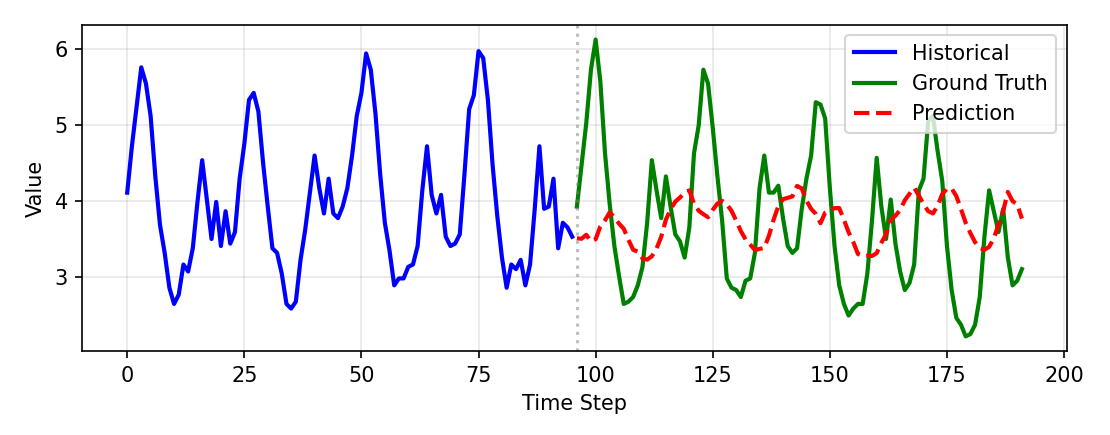
\includegraphics[width=\linewidth]{figures/prediction_sample_noCondition.eps}
% 	\caption{Prediction Result Based on MR- CDM model without conditional information}
% 	\label{fig:unconditional}
% \end{figure}

% To visually demonstrate the crucial role of conditional information in the diffusion model, \autoref{fig:result} and \autoref{fig:unconditional}  respectively show the performance of the unconditional diffusion model and the proposed conditional diffusion model in the same time series prediction task. Here, the blue solid line represents the historical observed sequence (0–95 steps) as input, the green solid line represents the true values (Ground Truth, 96–191 steps), and the red dashed line represents the model's prediction results. From the figures, it can be seen that under the unconditional setting, although the model can capture the overall trend, there are significant deviations in terms of detail fluctuations, peak responses, and temporal alignment, especially in the rapidly changing areas, indicating its lack of the ability to precisely model the temporal dynamic structure. 

% In contrast, after introducing conditional information, the model can more accurately track the intense fluctuations and local features of the true signal, and the prediction curve closely matches the true values, significantly enhancing the ability to restore short-term fluctuations and maintain long-term consistency. This comparison fully validates the effectiveness of the conditional mechanism in guiding the diffusion process and enhancing time-dependent modeling, further highlighting the superior performance of the proposed method in complex time series prediction tasks.

% \begin{table}[h]
% \centering
% \caption{Ablation Studies on Synthetic ETTh1}
% \label{tab:ablation_synthetic}
% \begin{tabular}{lccc}
% \hline
% Model-Variant & MSE & MAE & RMSE \\ \hline
% Baseline-NoDecomposition & {108.5863} & {8.0619} & {10.4204} \\
% UnconditionalDiffusion & {116.4437} & {8.3155} & {10.7909} \\
% NoImageFusion & {111.8180} & {8.2349} & {10.5744}\\
% FullModel & {1.2544} & {0.9080} & {1.1200 }\\
% \hline
% \end{tabular}
% \end{table}
% As shown in \autoref{tab:ablation_synthetic},we further conducted ablation studies on the synthetic dataset, and the results consistently demonstrate that each component of MR-CDM plays a vital role: multi-scale trend decomposition effectively captures hierarchical temporal patterns, conditional diffusion leverages historical context for accurate generation, and the image-based fusion mechanism enables meaningful integration of multi-scale features. Removing any one of these components leads to a significant performance drop, confirming that the full architecture is necessary and well-designed.

% \subsubsection{Second Ablation Study}
% To systematically evaluate the structural effectiveness of the proposed MR-CDM in multi-scale time-series modeling, we conduct an ablation study on the trend decomposition module. The experiments are performed on the LUFL variable of the ETTh1 dataset under a unified setting of prediction length, with MSE, MAE, and RMSE adopted as evaluation metrics. Specifically, three configurations are compared: the full MR-CDM model, MR-CDM w/o Trend1 (removing the low-frequency trend component), and MR-CDM w/o Trend3 (removing the high-frequency component). The reason for not removing Trend2 is that it is not the "highest frequency" nor the "smoothest", but somewhere in between, mainly carrying medium-term structural information.


% The results show that the full model achieves the best performance across all three metrics. Removing either trend component leads to a noticeable degradation in prediction accuracy, with a larger drop observed when Trend3 is removed. This indicates that the high-frequency component is critical for short-term fluctuation modeling, while the low-frequency component remains indispensable for preserving global trend dynamics. Overall, the proposed multi-scale trend decomposition mechanism enables collaborative modeling of short-term disturbances and long-term evolution within a unified framework, thereby improving model robustness and generalization in practical forecasting scenarios.


% \begin{table}[h]
% \centering
% \caption{Trend Decomposition Ablation Result}
% \label{tab:ablation_trendDecomposition}
% \begin{tabular}{lccc}
% \hline
% Model-Variant & MSE & MAE & RMSE \\ \hline
% MR-CDM w/o Trend1 & {1.9342} & {1.1247} & {1.3907} \\
% MR-CDM w/o Trend3 & {2.2769} & {1.2678} & {1.5089} \\
% FullModel & {1.4842} & {0.9650} & {1.2183}\\
% \hline
% \end{tabular}
% \end{table}



